\chapter{骨髓血细胞检测与识别软件设计}
本节介绍基于深度学习的骨髓血细胞检测与识别软件的设计。首先分析了软件的需求,包括了功能性需求
与非功能性需求。接着,介绍了软件的架构设计与各个模块的流程图与数据库表设计。软件模块包括了用户登录注册模块、骨髓血细胞检测模块、
骨髓血细胞识别模块、患者数据管理模块与日志模块。最后展示了软件实际实现的功能界面,并设计相关测试用例对软件功能进行测试。


\section{需求分析}
本节的目的是实现一个骨髓血细胞自动化检测识别软件,通过第三、四章介绍的深度学习算法将血细胞硬件采集设备收集的图像自动完成血细胞的定位、分类计数。
最终根据FAB分类标准给出病情的诊断。本软件主要解决人工镜检流程复杂、枯燥、主观性强等问题。医生可以将患者数据一键上传,在患者信息管理界面可以查询
相关患者的单张血细胞图像分类结果与整体血细胞分布的柱状图,此外还可以对错分类的血细胞重新进行标注。上述血细胞数据均落入到云端的数据库中,通过数据的不断积累,
未来可以进一步提升模型的识别性能。

\subsection{功能需求分析}
骨髓血细胞检测识别软件包含以下的几种功能,用户登录/注册功能、骨髓血细胞图像上传/检测功能、骨髓血细胞图像识别功能、
患者数据管理查看分析功能。

\textbf{1)用户登录/注册功能}

软件的首页为登录页,用户只有登录后才能使用网站的全部功能。注册用户仅为医院医生,注册后可以使用骨髓血细胞检测、
骨髓血细胞识别功能,并能对检测识别结果进行修订与更改。医生注册后可以对个人信息如昵称、电话、邮箱、部门、性别进行修改。

\textbf{2)血细胞检测功能}

医生输入患者的ID后,将扫描设备拍摄的骨髓血细胞数字化图像上传,上传后图像可在界面实时显示,并展示检测到的血细胞切片,
提供切片图像压缩包下载的功能。在检测精度方面,交并比(IOU)为0.75时,检测的平均精度(AP75)不低于0.90。
在IOU阈值为0.50~0.95时,检测平均精度(AP50:75)不低于0.85。


\textbf{3)血细胞识别功能}

医生在输入患者ID后,选择切片图像上传,软件可以将识别的结果呈现给医生。在识别精度方面,整体分类正确率不低于0.90
针对常见的骨髓血细胞类型如嗜中性粒细胞,淋巴、红细胞的f1-score大于0.95。

\textbf{4)患者数据管理分析功能}

医生可以搜索某患者的骨髓血细胞图像切片,并展示算法识别的类别,医生可以对血细胞识别的类别进行修改,并人工确认。
软件可以对患者的血细胞类别数量分布以直方图或饼状图的形式进行展现,根据FAB标准对血液疾病类型给出初步诊断结果。

\subsection{非功能需求分析}
软件的非功能性需求主要包含以下几个方面。1)性能与速度,需要每小时可完成20张涂片约2000个骨髓血细胞的检测与识别。
2)数据安全性与可靠性,数据计算时,需要保证算法的正确与稳定性,使用数据库维护与更新数据,保证数据的完整性和可追溯性。
3)软件的稳定性,软件在使用中不会因为某些异常或错误而崩溃或无法正常运行。4)软件的易用性,软件的界面与交互设计应该用户友好,
用户能够方便的使用软件骨髓血细胞检测识别任务。5)软件的可扩展性,有清晰的模块化与接口化设计,可以方便的进行检测识别算法的升级。
架构上采用可扩展的架构,可方便的支持新增功能。

\section{软件设计}

\subsection{软件架构设计}
骨髓血细胞检测与识别软件开发使用的技术框架为B/S架构。开发环境为Windows 10、前端使用Vue框架与Element UI组件库。
后端使用的框架Django 2.4、深度学习模型部署工具ONNX、数据库为Mysql 8.0。

\begin{figure}[htbp]                     
  \centering                      
  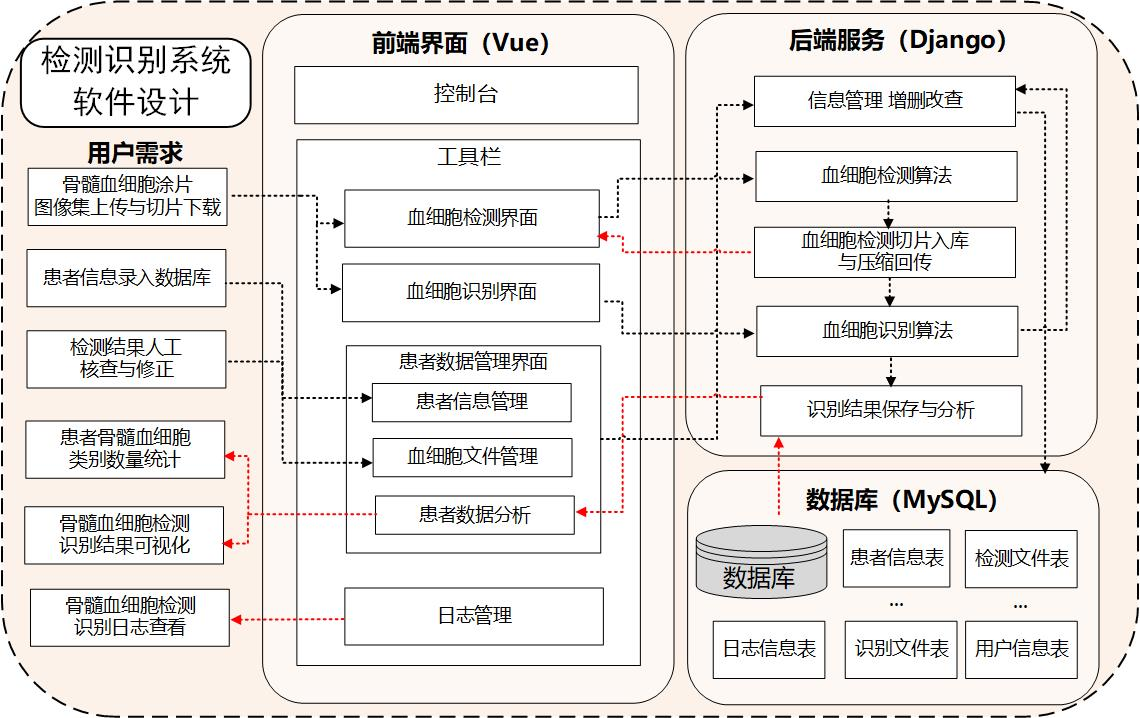
\includegraphics[width=0.99\linewidth]{software_structure.jpg}                      
  \caption{骨髓血细胞检测识别软件架构图}                      
  \label{fig:software}       
\end{figure}
骨髓血细胞检测识别架构如图~\ref{fig:software}所示,根据用户需求分析,主要划分为四个模块分别是用户模块、骨髓血细胞检测模块、
骨髓血细胞识别模块与患者数据管理模块。

软件采用前后端分离的架构,分别进行独立开发与部署。前端与后端的数据交互与通信使用axios网络请求库。
后端服务部署在GPU服务器上,前端服务可以部署在CDN或者云服务器上,可以方便的进行系统升级、扩容与扩展。
软件无需用户进行安装,打开浏览器输入网页域名即可使用,具有非常好的跨平台性,在windows、mac、linux
操作系统下均可使用。数据与计算服务均在云端实现,降低了对使用者计算机本地资源的依赖。

\subsection{软件数据库设计}
数据库是骨髓血细胞检测识别软件中的重要部分,其用于存储与管理血细胞数据,为医生提供方便快捷的数据查询、修改与更新等功能。
MySQL是一个开源且功能强大的关系型数据库管理系统,支持并发读写,可以处理大规模数据,可靠性强,能够保证数据的完整性与安全性,
因此我们使用MySQL数据库\cite{christudas2019mysql}用于软件的数据存储与管理。

软件数据库表主要包括了用户信息表、检测文件表、识别文件表、日志表等,其设计的合理性对于软件性能稳定性与可扩展性至关重要,
下面将对各数据表设计进行详细介绍。

1)用户信息表,用户信息表如表~\ref{table:user_table}所示,其记录了用户基本信息如用户名、密码、头像、邮箱、手机等。用户密码通过MD5加密算法生成一个长度为128位的哈希值存储在数据库中,
在登录时,通过比较用户密码的哈希值是否相同对用户进行校验。用户登录后可以对自己的个人信息进行修改。超级用户如医生可以对骨髓血细胞检测与识别的结果进行人工核对与修改。
\begin{table}
    \caption{用户信息表}   
    \centering 
    \label{table:user_table}
    % \begin{tabular}{cccc}
    \begin{tabular*}{0.9\hsize}{@{}@{\extracolsep{\fill}}cccc@{}}
      \toprule[1pt]
      字段名称  &  数据类型 & 约束条件 & 字段说明 \\
      \midrule[1pt] 
      id & INTEGER & 主键/自增 & 唯一用户ID   \\ 
      username & varchar(150) & 非空 & 用户名(登录)   \\ 
      password & varchar(128) & 非空 & 用户登录密码   \\ 
      email    & varchar(255) & 非空 & 用户邮箱 \\
      nickname & varchar(40)  &  -   & 用户昵称  \\ 
      mobile   & varchar(255) &  -   & 用户电话  \\
      avatar   & varchar(255) &  -   & 用户头像  \\
      gender   & INTEGER      &  -   & 用户性别   \\
      dept\_id  & bigint       &  外键   &  部门ID  \\ 
      create\_datetime & datetime & -    & 用户创建时间 \\
      update\_datetime & datetime & -    & 最近一次修改时间 \\
      last\_login & datetime & -           & 最近一次登录时间 \\
      is\_superuser & bool   &  -         & 是否超级用户 \\
      \bottomrule[1pt]      
    \end{tabular*} 
  \end{table}

2)检测文件表,表~\ref{table:detect_table}为检测文件表,该表用于存储医生上传的患者骨髓血细胞图像以及检测算法检测到的血细胞的坐标。
首先根据上传的文件内容根据MD5算法计算出文件的128位哈希值,并将该名称作为文件名称落入到数据库中。血细胞检测结果坐标以
json字符串的形式进行存储。
\begin{table}
    \caption{检测文件表}   
    \centering 
    \label{table:detect_table}
    % \begin{tabular}{cccc}
    \begin{tabular*}{0.9\hsize}{@{}@{\extracolsep{\fill}}cccc@{}}
      \toprule[1pt]
      字段名称  &  数据类型 & 约束条件 & 字段说明 \\
      \midrule[1pt] 
      id           & INTEGER      & 主键/自增    & 唯一文件ID   \\ 
      filename     & varchar(200) & 非空         & 上传图像名称   \\ 
      url          & varchar(100) & 非空         & 文件存储路径   \\ 
      md5sum       & varchar(36)  & 非空         & 文件MD5哈希值 \\
      patien\_id   & bigint       & 非空         & 患者ID  \\ 
      creator\_id  & bigint       & 外键         & 上传者ID  \\ 
      create\_datetime & datetime & -    & 上传时间 \\
      update\_datetime & datetime & -    & 最近一次修改时间 \\
      description      & varchar(1024) & - & 检测结果json描述 \\
      \bottomrule[1pt]      
    \end{tabular*} 
  \end{table}

3)识别文件表,表~\ref{table:recog_table}为识别文件表,该表用于存储医生上传的患者骨髓血细胞切片图像与识别的血细胞类别信息。
根据上传的文件内容根据MD5算法计算出文件的128位哈希值,并将该名称作为文件名称落入到数据库中。is\_confirmed字段
表示该条识别结果是否被医生工人核对。
\begin{table}
    \caption{识别文件表}   
    \centering 
    \label{table:recog_table}
    % \begin{tabular}{cccc}
    \begin{tabular*}{0.9\hsize}{@{}@{\extracolsep{\fill}}cccc@{}}
      \toprule[1pt]
      字段名称  &  数据类型 & 约束条件 & 字段说明 \\
      \midrule[1pt] 
      id           & INTEGER      & 主键/自增    & 唯一文件ID   \\ 
      filename     & varchar(200) & 非空         & 上传图像名称   \\ 
      url          & varchar(100) & 非空         & 文件存储路径   \\ 
      md5sum       & varchar(36)  & 非空         & 文件MD5哈希值 \\
      cell\_id      & INTEGER      & -            & 骨髓血细胞类别ID  \\
      cell\_name    & varchar(200) & -            & 骨髓血细胞名称  \\
      patien\_id   & bigint       & 非空         & 患者ID  \\ 
      creator\_id  & bigint       & 外键         & 上传者ID  \\ 
      create\_datetime & datetime & -    & 上传时间 \\
      update\_datetime & datetime & -    & 最近一次修改时间 \\
      is\_confirmed    & bool     & -    & 是否人工核对 \\
      \bottomrule[1pt]      
    \end{tabular*} 
\end{table}
\section{各个模块设计}
本节将详细介绍四大模块的计算流程设计与UI界面设计。用户主界面如图~\ref{fig:interface}所示,
界面左侧为工具栏,功能选项有控制台、骨髓血细胞检测、骨髓血细胞识别、患者数据管理与日志管理。患者数据管理菜单下
有三个子菜单分别是患者信息管理、患者数据分析、血细胞文件管理。Tab栏展示了当前界面所属的窗口,可以方便的
进行不同功能页面的切换。主窗口显示用户的操作界面,展示用户上传的骨髓血细胞数据与检测识别的结果,并将患者
骨髓血细胞的数据分布以柱状图或饼状图的形式展示。右上角的用户管理部分可查看与修改当前用户信息、注销当前用户登录,
系统通知消息也在此部分进行展示。
\begin{figure}[htbp]                     
  \centering                      
  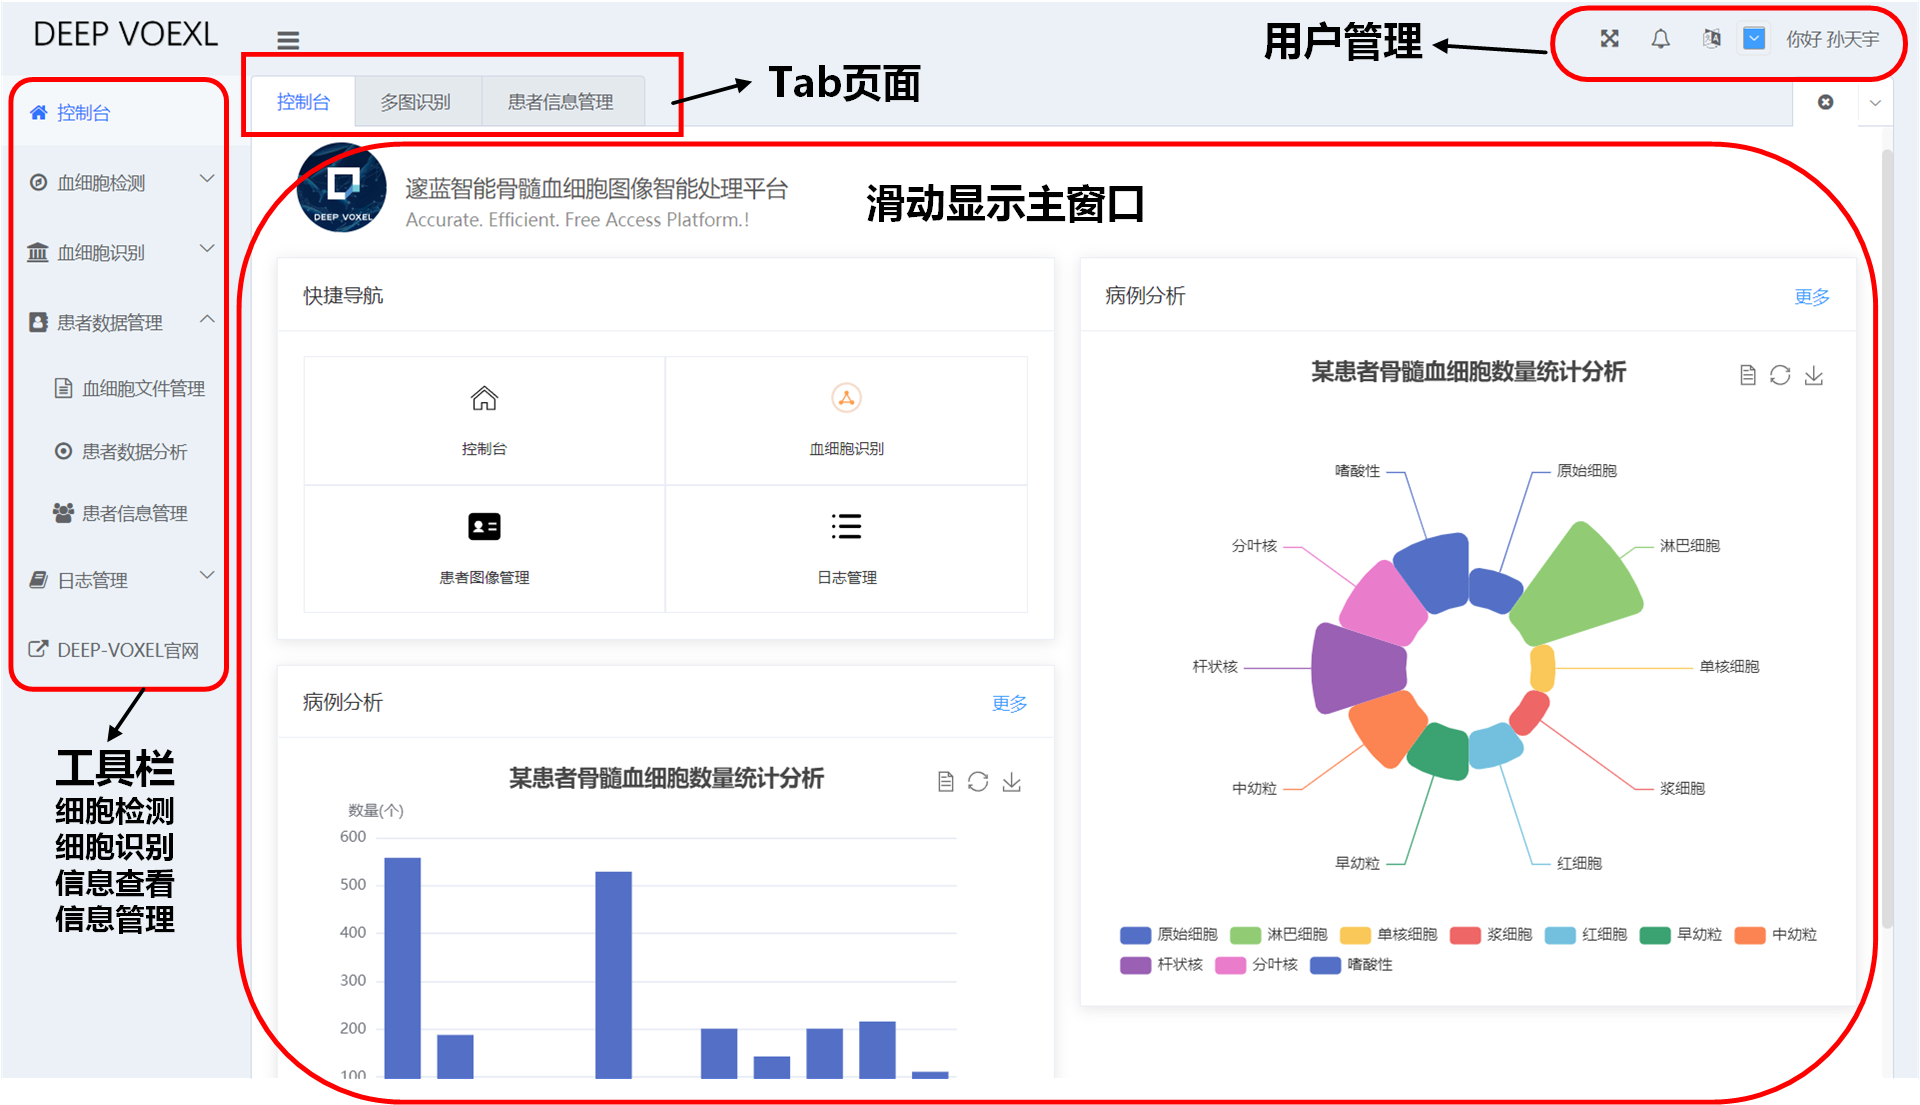
\includegraphics[width=0.90\linewidth]{console.png}                      
  \caption{骨髓血细胞检测识别软件界面}                      
  \label{fig:interface}       
\end{figure}
\subsection{用户模块}
用户登录与修改个人信息界面如图~\ref{fig:software_user}所示,用户模块是网站最基础的模块,用户在注册后,用户信息会写入数据库的用户信息表中,
在登录时需要填写注册时的用户名、密码与验证码信息,用户在点击登录按钮后,后端会对用户名与密码在数据库中进行核验,如果正确则会跳转到
软件的首页的控制台页面,否则会提示用户输入的用户名或密码错误。用户在登陆后,可以点击右上角的头像去修改并完善个人信息,如密码、电话、邮箱与昵称等。

\begin{figure}[htbp]
	\centering
	\begin{subfigure}{0.4\linewidth}
		\centering
		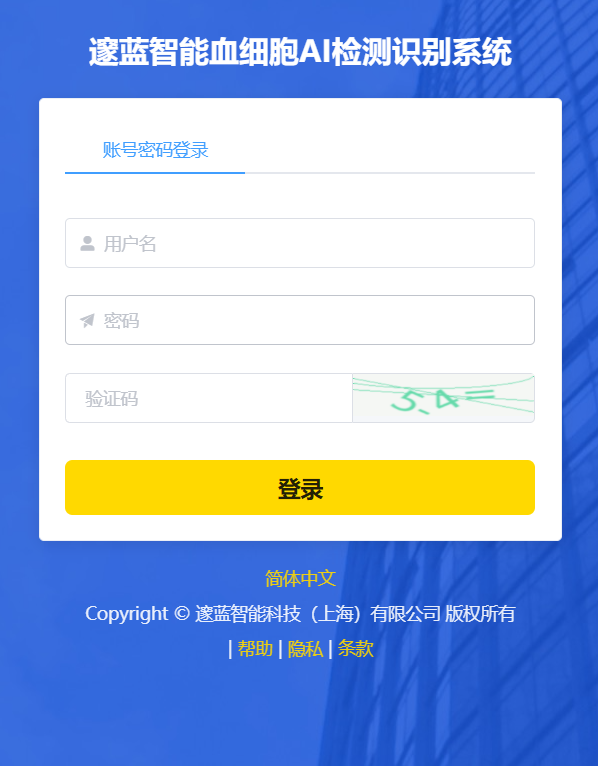
\includegraphics[width=0.95\linewidth, height=1.20\linewidth]{software/login.png}
    \caption{用户登录页}
	\end{subfigure}
	\centering
	\begin{subfigure}{0.40\linewidth}
		\centering
		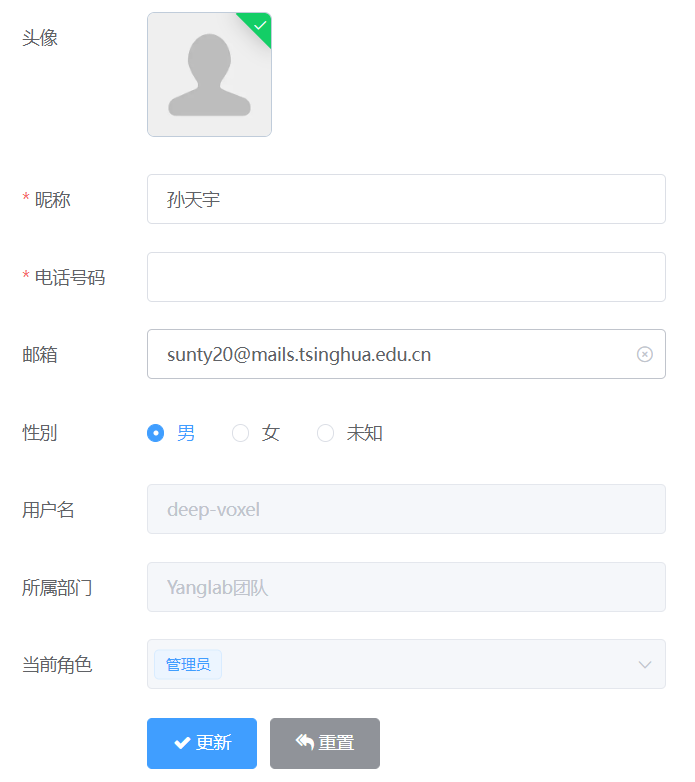
\includegraphics[width=0.95\linewidth, height=1.20\linewidth]{software/update.png}
    \caption{用户信息修改页}
	\end{subfigure}
  \caption{用户模块界面示意图}
	\label{fig:software_user}
\end{figure}
\subsection{骨髓血细胞检测模块}
骨髓血细胞检测界面如图~\ref{fig:interface_detect}所示,首先需要填写患者ID,然后点击“+”号,上传患者骨髓血细胞图像,
该过程调用后端$\text{/api/system/detect\_file}$接口,将细胞图像写入到数据库中,调用成功后将文件的url列表返回前端。然后点击检测按钮
调用后端$\text{/api/recognition/save\_detect}$接口,传输参数为待检测的url文件列表,后端调用基于ONNX部署的改进的RetinaNet骨髓血细胞
检测模型,然后将检测得到的坐标信息返回给前端,在检测结果区域以红色框进行标出。最后可以点击下载切片按钮,获得剪切后的血细胞图像切片文件。
\begin{figure}[htbp]                     
  \centering                      
  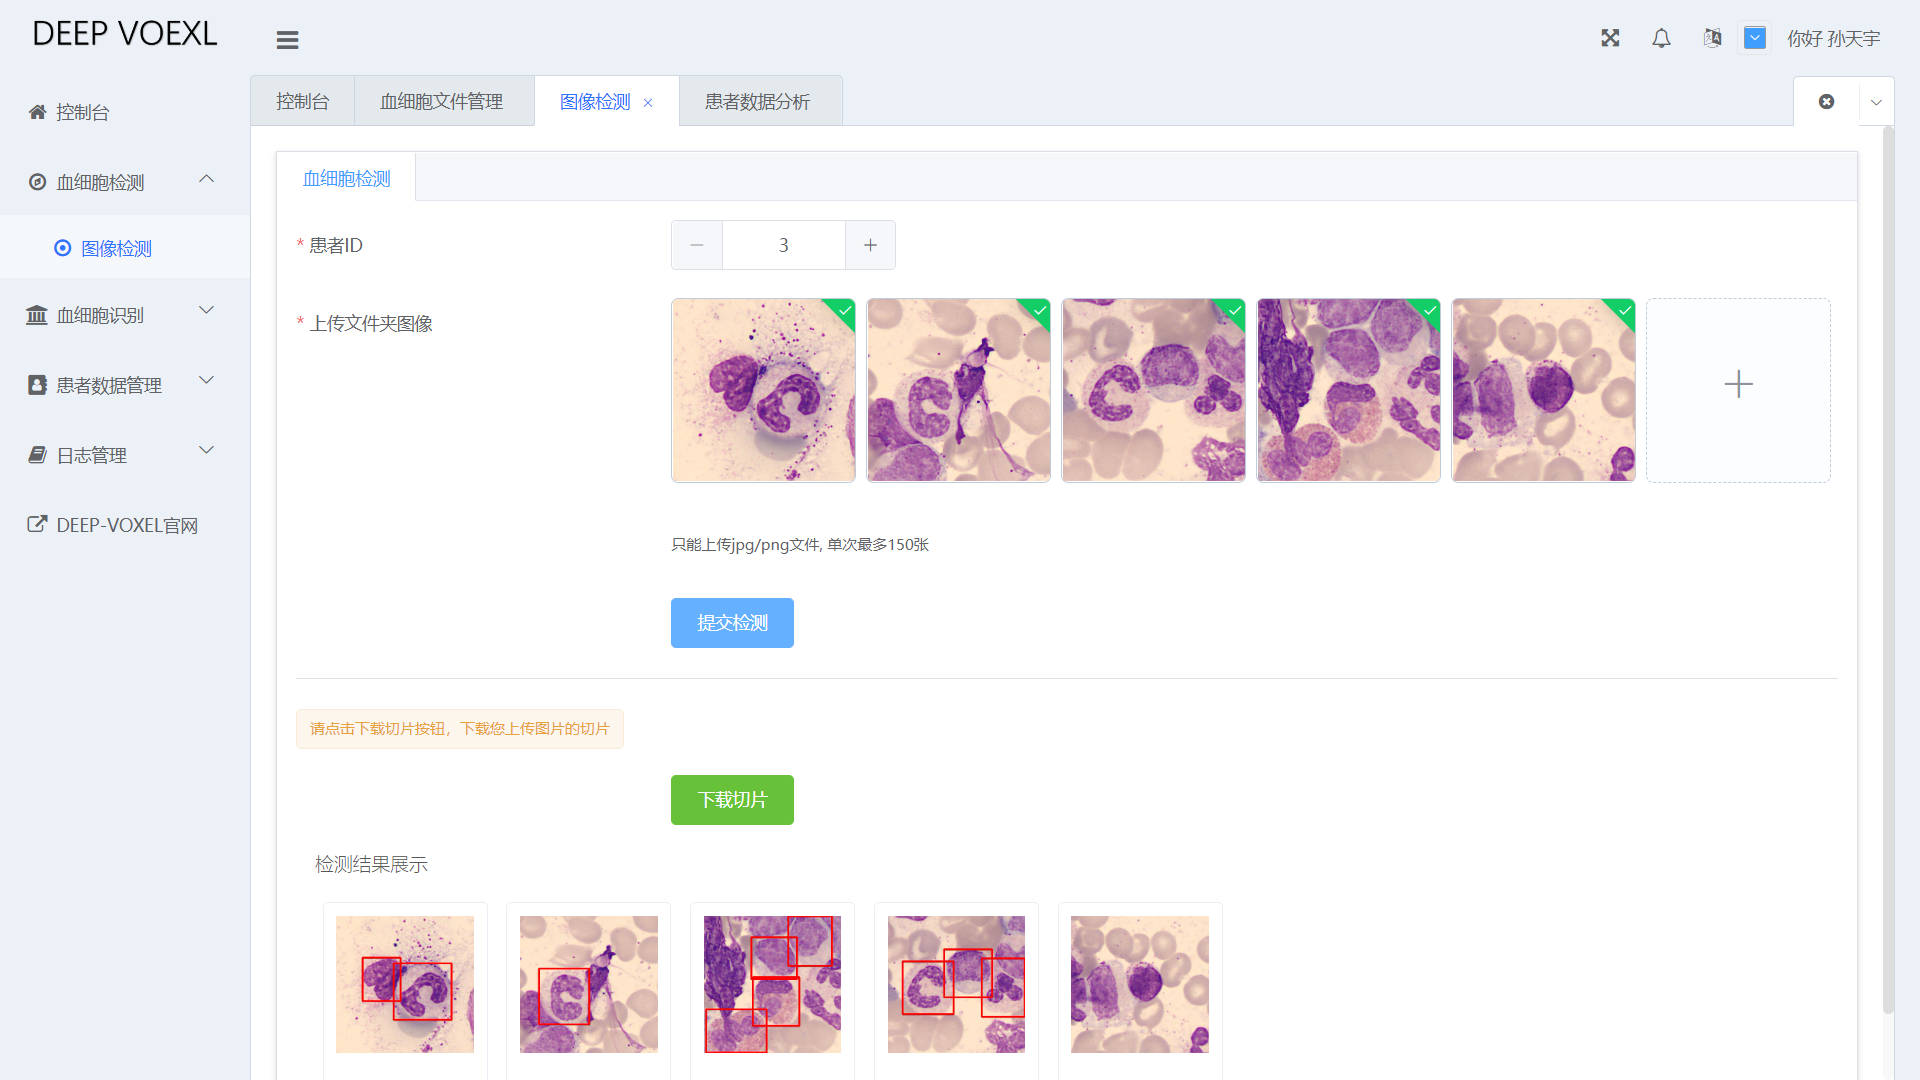
\includegraphics[width=0.90\linewidth]{software/detect.png}                      
  \caption{骨髓血细胞检测界面}                      
  \label{fig:interface_detect}       
\end{figure}
\subsection{骨髓血细胞识别模块}
骨髓血细胞识别界面如图~\ref{fig:interface_recog}所示,首先输入患者的ID,接着点击“+”号,选取检测部分下载的骨髓血细胞
切片图像,类似骨髓血细胞检测界面部分,图像会存储到数据库中。点击识别提交按钮,后端会调用ONNX部署的改进Vision Transformer模型
对骨髓血细胞类别进行识别,将血细胞的类别与名称以json串的形式返回,前端在页面下方的文本框中会按照上传图像的顺序显示
各个图像的类别编号与类别名称。每个血细胞的具体信息可以到患者数据管理菜单下的血细胞文件管理页面进行查看。
\begin{figure}[htbp]                     
  \centering                      
  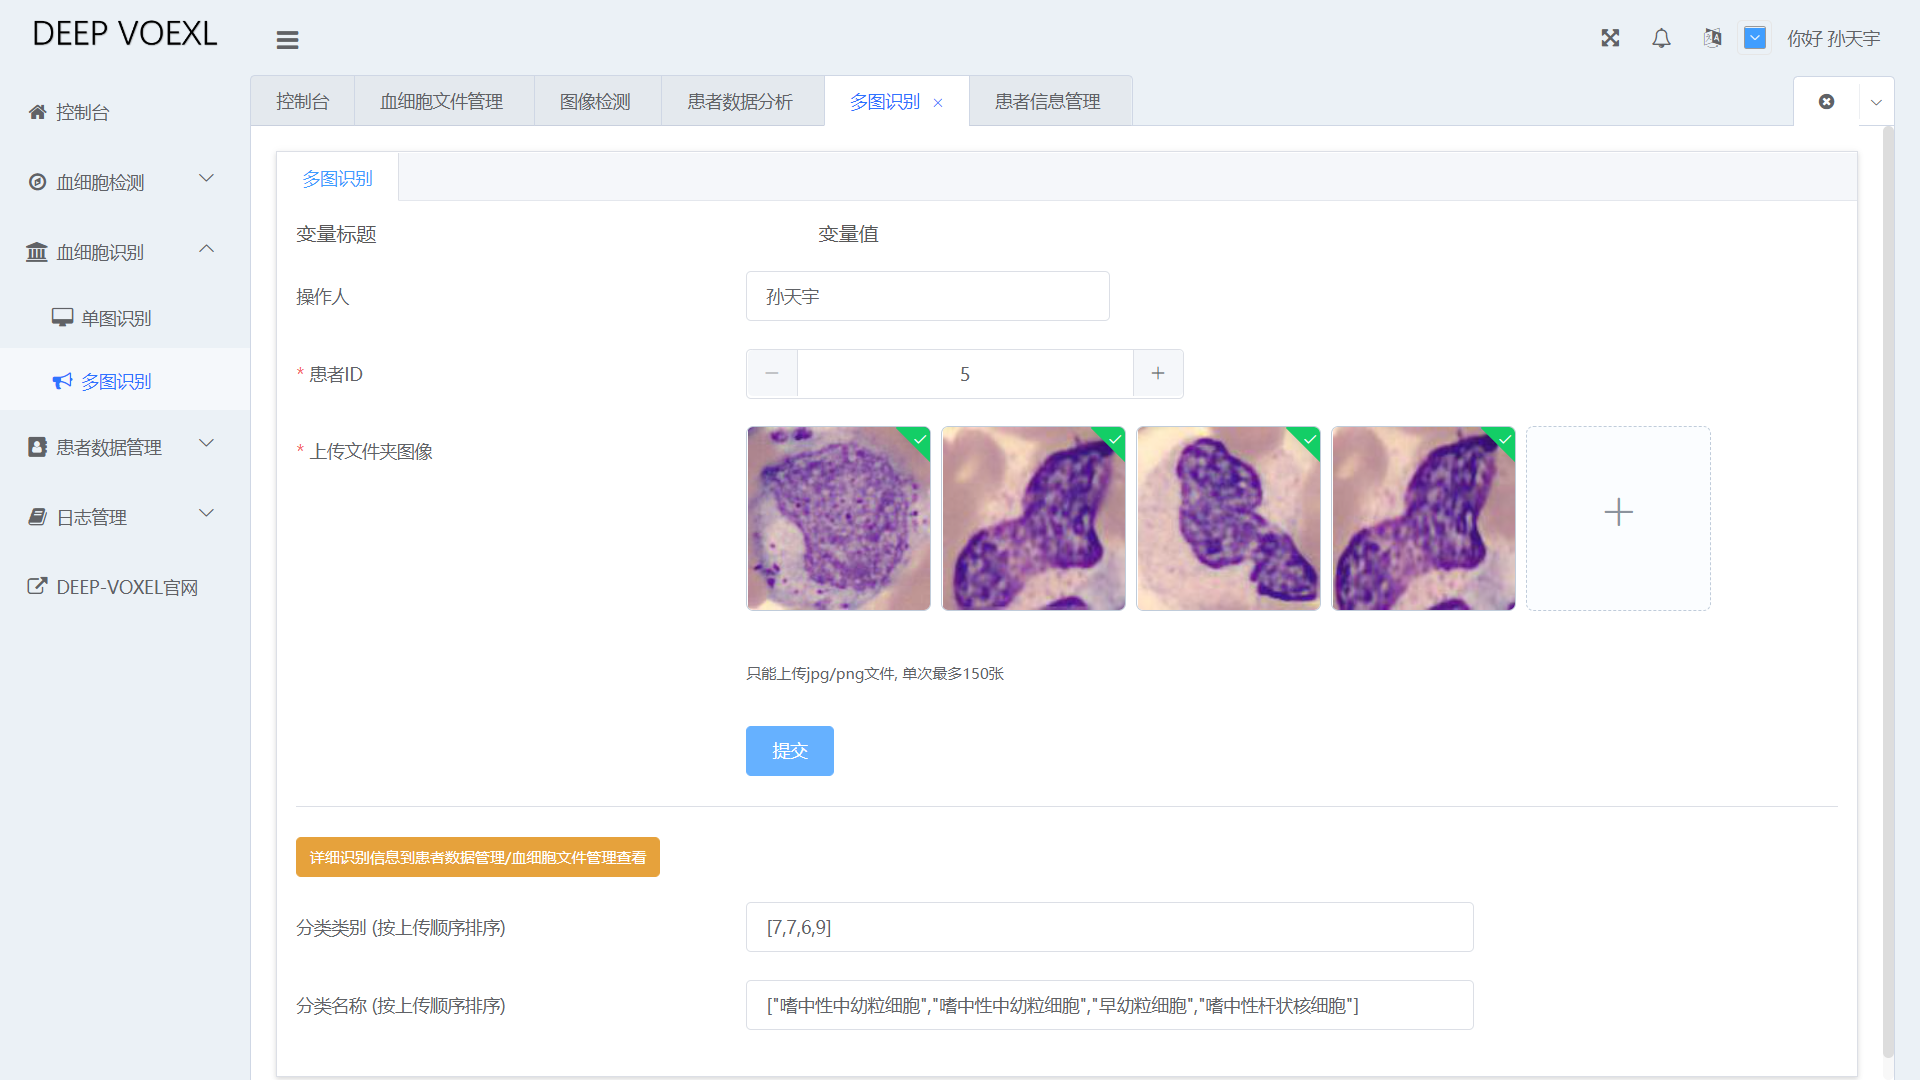
\includegraphics[width=0.90\linewidth]{software/recognition.png}                      
  \caption{骨髓血细胞识别界面}                      
  \label{fig:interface_recog}       
\end{figure}
\subsection{患者数据管理模块}
患者数据管理模块下总共有三个子页面,分别是血细胞文件管理页面、患者数据分析页面与患者信息管理页面。
\subsubsection{血细胞文件管理}
血细胞文件管理界面将骨髓血细胞识别界面上传的血细胞图像数据与识别结果以表格的形式进行展现,如图~\ref{fig:interface_result}所示,表格
从左到右列名分别是患者ID、文件名称、缩略图、血细胞类别、血细胞名称、上传/核验医师、是否人工确认、更新时间与操作。
点击血细胞类别下拉列表,可以对类别进行更改,同时自动更新血细胞名称。点击是否人工确认下拉列表选择true表示该条
数据已经通过人工确认。在最后的操作列,可以对血细胞其他信息进行编辑或者删除。
\begin{figure}[htbp]                     
  \centering                      
  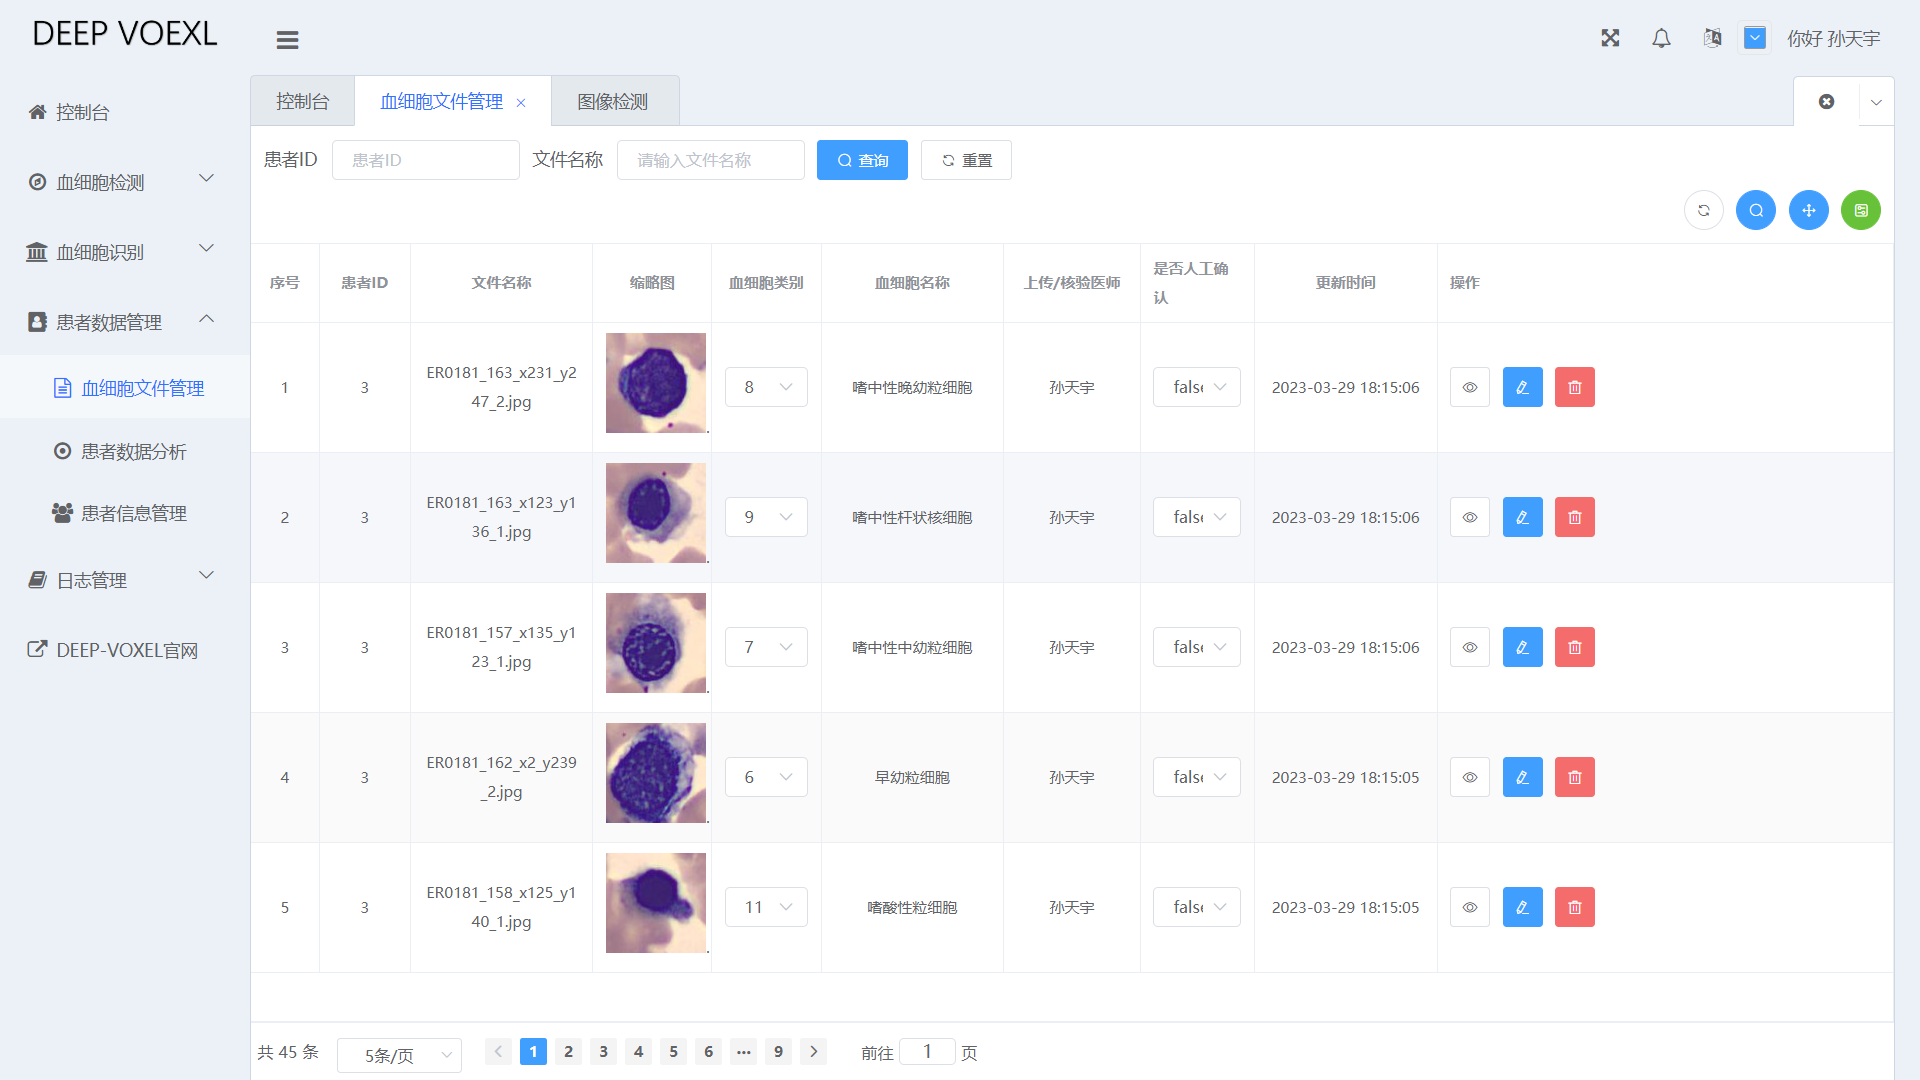
\includegraphics[width=0.9\linewidth]{software/result.png}                      
  \caption{医生核验识别结果界面}                      
  \label{fig:interface_result}       
\end{figure}
\subsubsection{患者数据分析}
患者数据分析界面如图~\ref{fig:interface_info}所示,输入患者ID,点击查询后,在下方患者详情的文本框中会以文本的形式展示各血细胞类别的
名称与数量。各类血细胞的分布以柱状图与饼状图的方式呈现给医生,辅助医生对白血病的类型进行诊断。
决策算法根据FAB(French-American-British)分型标准给出初步的白血病类型诊断建议。在FAB分类标准中,原始细胞占比大于30\%作为急性白血病的诊断标准,
根据原始细胞的类型分为急性淋巴细胞白血病(acute lymphoblastic leukemia,ALL)与急性髓系白血病(acute myeloid leukemia,AML)。当原始/幼稚
淋巴细胞占比超过50\%为ALL白血病。AML白血病根据不同细胞的占比分为M0$\sim$M7型,例如颗粒过多早幼粒细胞占比大于30\%,为M3型的急性早幼粒细胞白血病。
\begin{figure}[htbp]                     
  \centering                      
  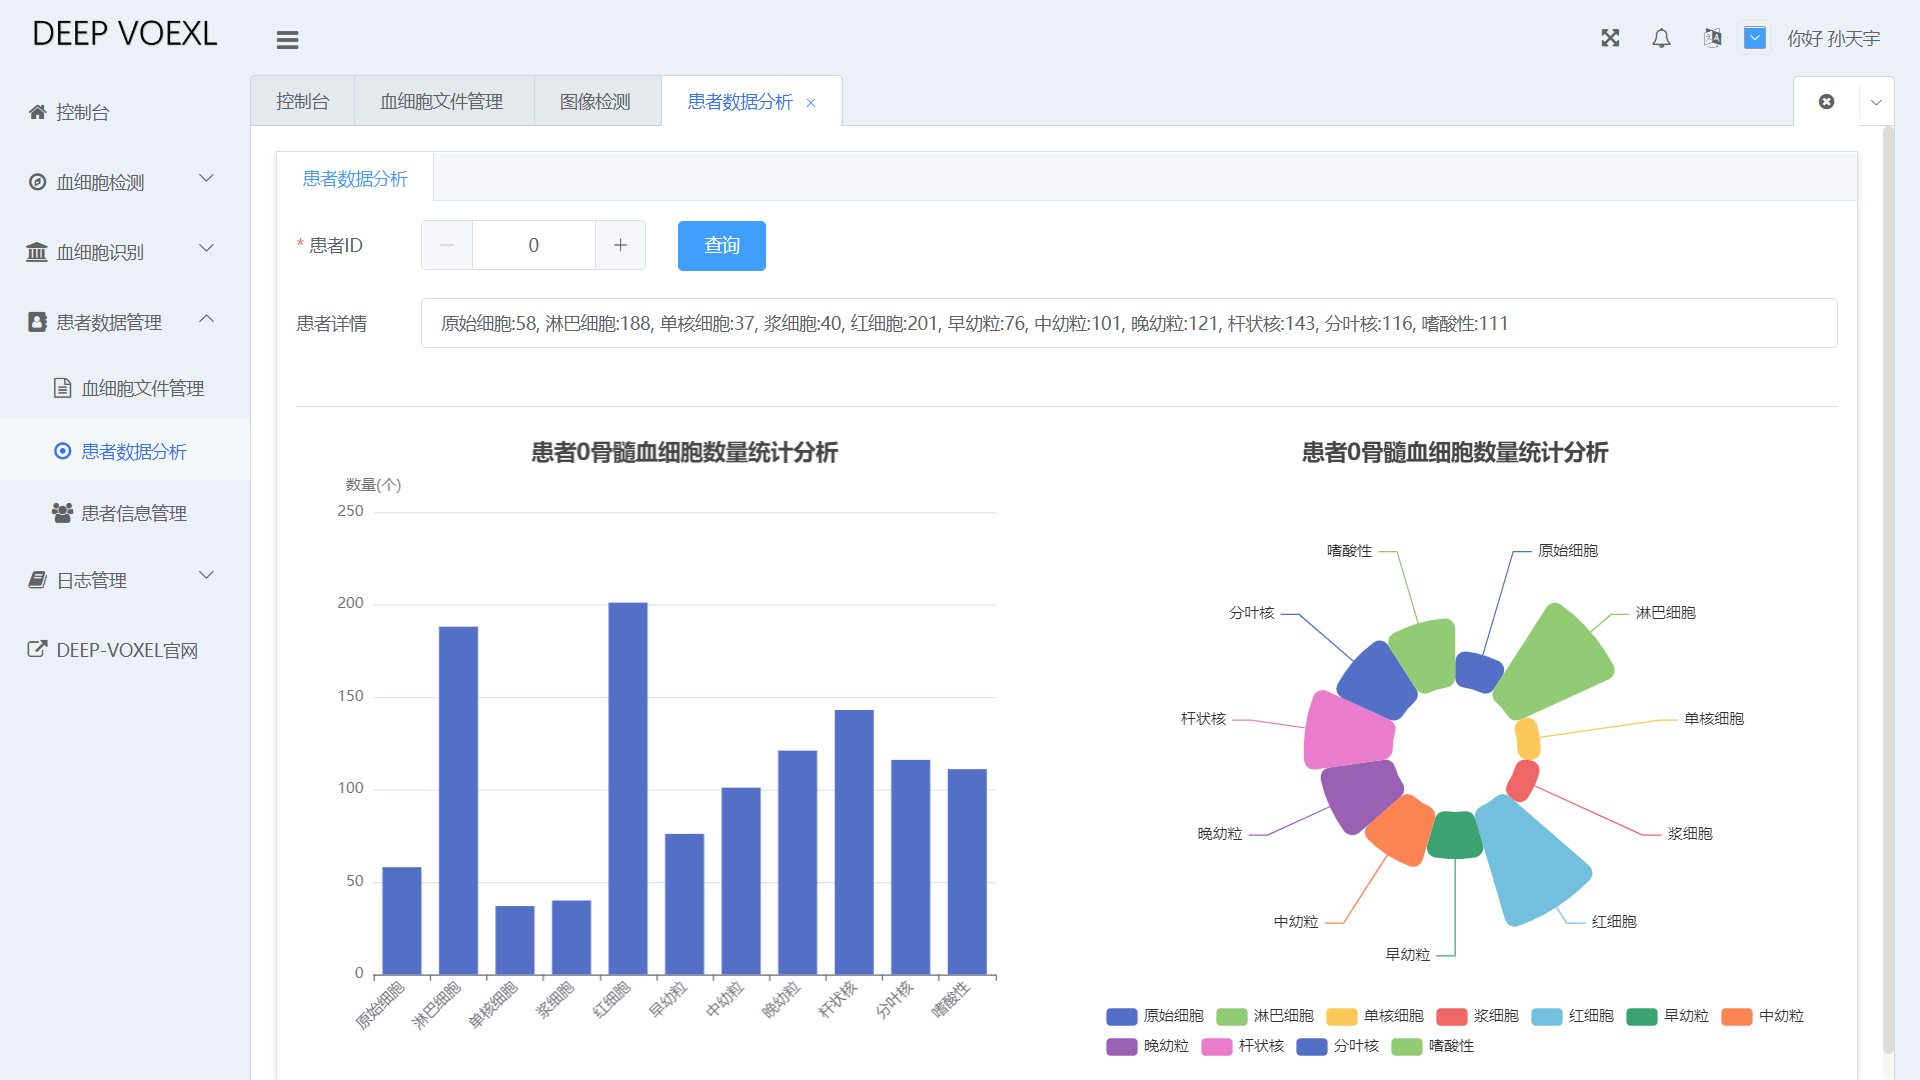
\includegraphics[width=0.9\linewidth]{software/info.png}                      
  \caption{患者数据分析界面}                      
  \label{fig:interface_info}       
\end{figure}
\subsubsection{患者信息管理}
患者信息管理界面如图~\ref{fig:interface_patient}所示,在该界面中医生可以新增、删除、编辑、导入与导出患者数据。
点击+新增按钮,弹出子页面中依次填入患者的姓名、性别、身份证号码等信息,点击确定即可完成患者信息的录入。在页面的最上方
可以根据姓名、关键词等信息进行患者信息的搜索。
\begin{figure}[htbp]                     
  \centering                      
  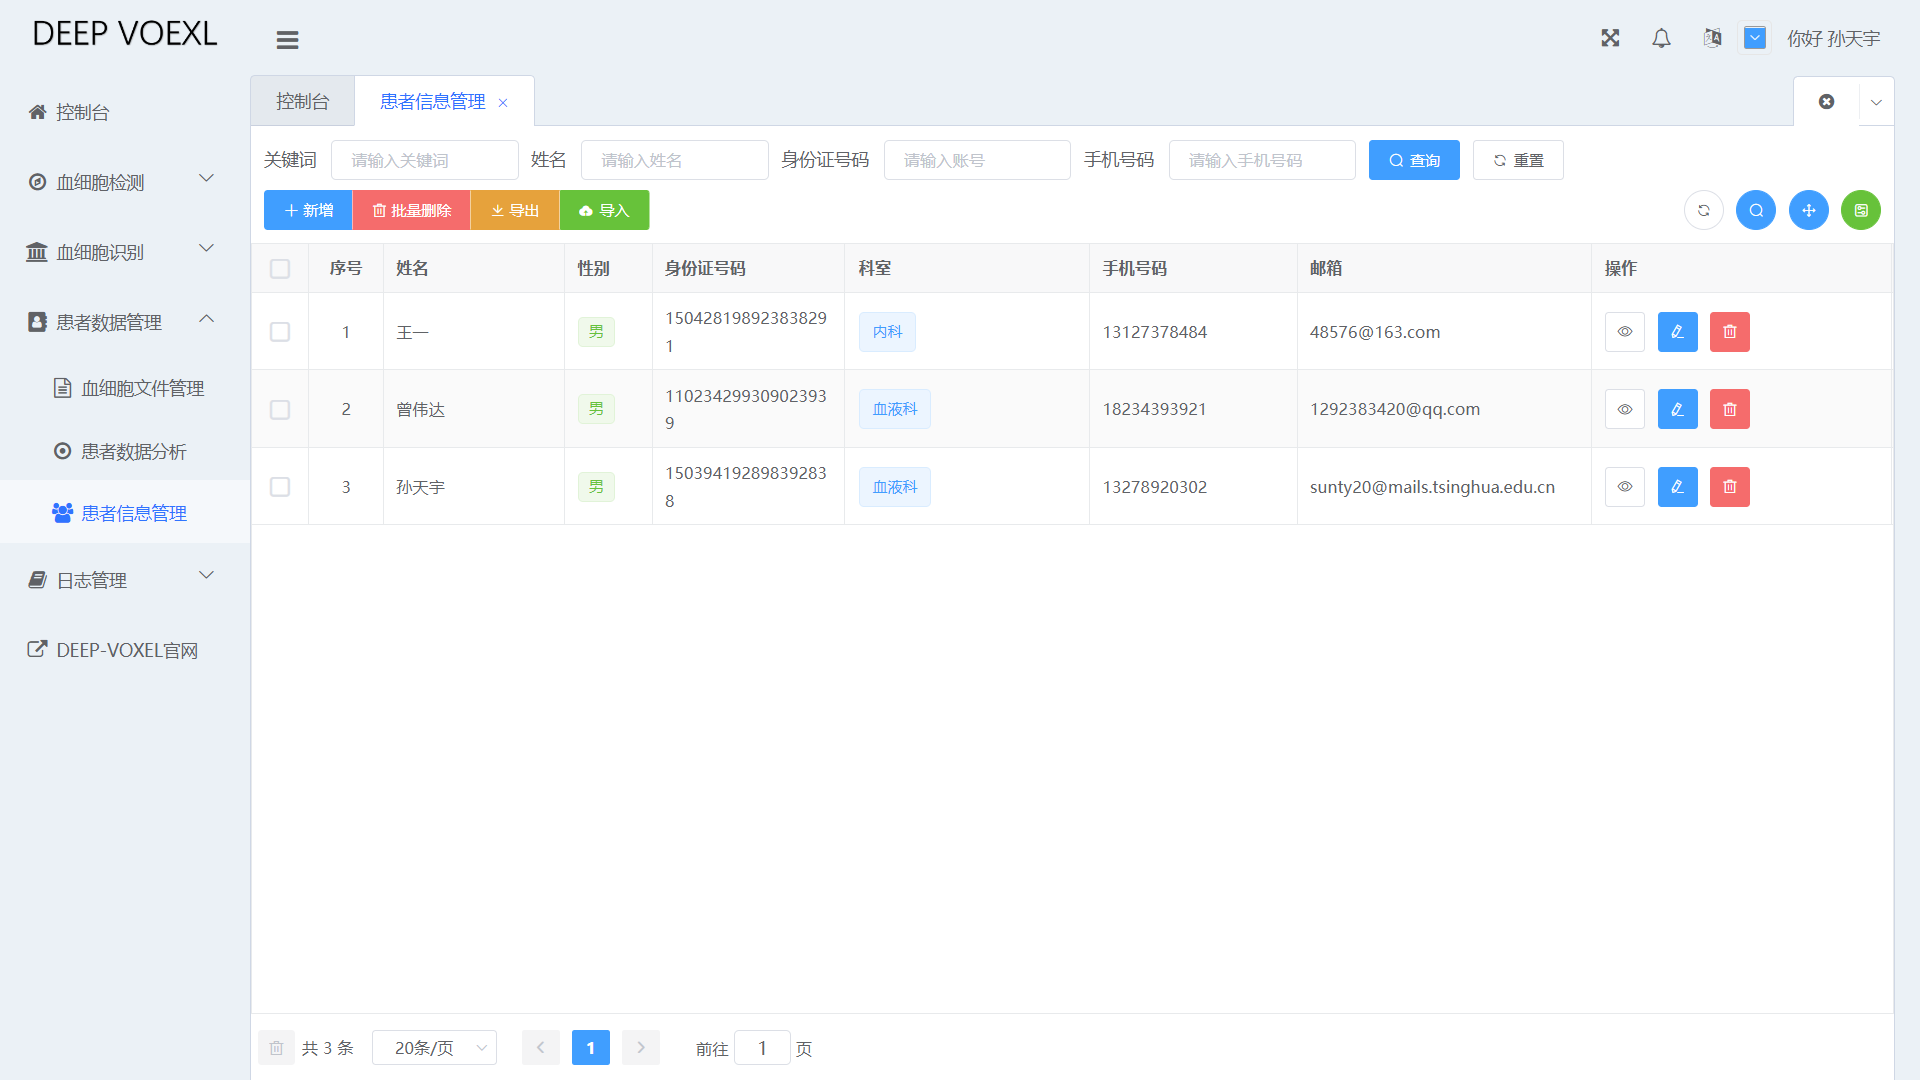
\includegraphics[width=0.9\linewidth]{software/patient.png}                      
  \caption{患者信息录入页面}                      
  \label{fig:interface_patient}       
\end{figure}
\section{小结}
本文基于B/S架构设计并开发了骨髓血细胞检测与识别软件。前端使用Vue框架与Element UI组件库。
后端使用的框架为Django2.4、深度学习模型部署工具使用ONNX进行模型部署、数据存储使用Mysql8.0。软件实现了用户模块、骨髓血细胞检测模块、
骨髓血细胞识别模块与患者数据管理模块。通过该软件,医生可以将将患者骨髓血细胞图像数据一键上传,软件自动完成血细胞的定位、分类计数,
医生可以查询相关患者的单张血细胞图像分类结果与整体血细胞分布的柱状图,并对血细胞类别进行校对与修改,软件最终根据FAB分类标给出诊断建议。
实测中,软件的运行速度与检测识别精度均达到了项目指标的要求,未来有望应用于白血病的临床辅助诊断。
